\documentclass[]{report}


% Title Page
\title{Homework I Solutions \\ of \\ \emph{Advanced Mechanical Vibrations} class.}
\author{Burak ER}
\usepackage{amsmath}
\usepackage{cleveref}
\usepackage{commath}
\usepackage{pst-all}
\usepackage{tikz}

\begin{document}


\maketitle
\begin{abstract}
Includes the solutions for the first homework problems of \emph{Advanced Mechanical Engineering} class given at Bursa Technical University, in fall semester 2013.
\\
\\
Written by \LaTeX ~using TeXstudio...
\end{abstract}
\section*{Solution of problem 1}
\subsection*{a)}
%\begin{figure}[!ht]
%    \centering
%    \begin{pspicture}[showgrid=false,xunit=4cm,yunit=1.2cm](-2,-2)(2,2)
%    %frames and zigzags
%      \psframe[linecolor=black](-1,-0.3)(1,0.3)
%	\pszigzag[doubleline=false,linecolor=black,coilheight=0.6,coilwidth=0.3,coilarmA=0.1,coilarmB=0.1,tbarsize=1.7]{-|}(-0.3,-0.3)(-0.3,-1)
%		  \rput{0}(-0.2,-0.6){\psframebox*{$k_1$}}
%		      \psframe[fillstyle=vlines,,linecolor=white](-0.5,-1)(-0.1,-1.3)
%	\pszigzag[doubleline=false,linecolor=black,coilheight=0.6,coilwidth=0.3,coilarmA=0.1,coilarmB=0.1,tbarsize=1.7]{-|}(0.3,0.3)(0.3,1)
%	   \psframe[fillstyle=vlines,linecolor=white](0.1,1)(0.5,1.3)
%      \psframe[linecolor=black](0.99,-1)(1.6,1)
%      \rput(1.3,0){\psframebox[linecolor=white]{m}}
%	   \rput{180}(-1.1,0){\psframe[fillstyle=vlines,linecolor=white](-0.05,-0.8)(0.05,0.8)}
%	   	   \psline(-1.,-0.3)(-1,0.8)
%		\pswedge(-1.05,0){0.6}{-90}{90}
%		\pscircle(-1,0){0.2}
%		  \rput{0}(0.4,0.6){\psframebox*{$k_2$}}
%		  %dimensions
%		  	   \psline(-1.,-0.3)(-1,0.8)
%		  \psline{<->}(-1,2)(1,2)
%		  \psline{<->}(-1,1.5)(0.3,1.5)
%		  \psline{<->}(-1,1)(-0.3,1)
%		  \psline{-}(-1,0.8)(-1,2)
%		  \psline{-}(-0.3,0.3)(-0.3,1)
%		  \psline{-}(0.3,1.3)(0.3,1.8)	
%		  \psline{-}(0.99,1)(0.99,2)	
%		  \rput{0}(-0.65,1){\psframebox*{$a$}}
%		  \rput{0}(-0.35,1.5){\psframebox*{$b$}}		 	  		  	  		 	  
%		  \rput{0}(0,2){\psframebox*{$l$}}  
%    \end{pspicture}
%    \caption{Problem 1's drawing}
%  \end{figure}
 \begin{figure}[ht!]
\centering
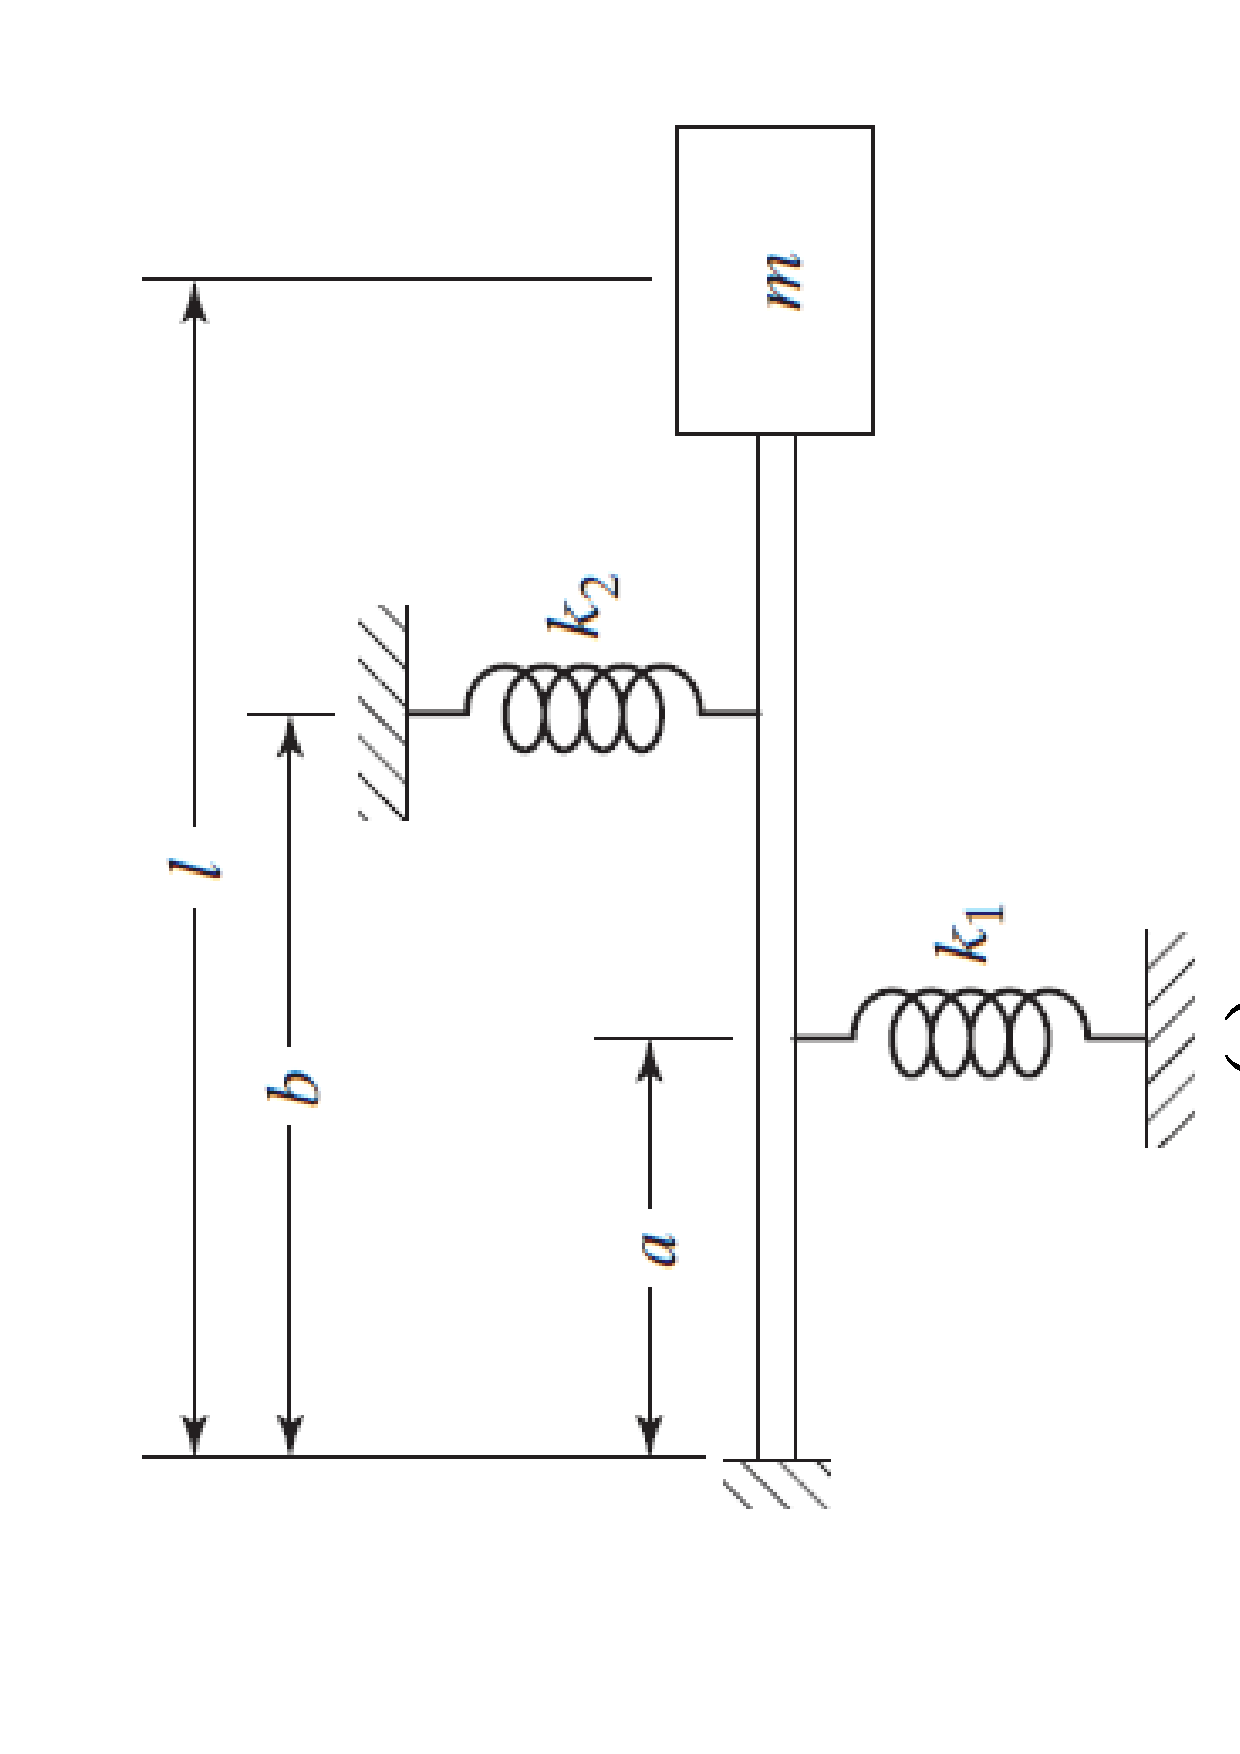
\includegraphics[width=0.7\linewidth,angle=-90]{./problem1a}
\caption[Drawing of Problem 1(a)]{Drawing of Problem 1(a)}
\label{fig:problem1}
\end{figure}
~\\ 
\textbf{Equations of motion using Newton's approach:}\\
\\
We should write translational displacements of points on the rod in terms of rotation of the rod. Therefore, for small angles
\begin{figure}[!ht]
    \centering
    \begin{pspicture}[showgrid=false,xunit=3.5cm,yunit=1cm](-1,-2)(3,2)
    %first situation
          \psframe[linecolor=black](-1,-0.3)(1,0.3)
    	\pszigzag[doubleline=false,linecolor=black,coilheight=0.6,coilwidth=0.3,coilarmA=0.1,coilarmB=0.1,tbarsize=1.7]{-|}(-0.3,-0.3)(-0.3,-1)

    		      \psframe[fillstyle=vlines,,linecolor=white](-0.5,-1)(-0.1,-1.3)
    	\pszigzag[doubleline=false,linecolor=black,coilheight=0.6,coilwidth=0.3,coilarmA=0.1,coilarmB=0.1,tbarsize=1.7]{-|}(0.3,0.3)(0.3,1)
    	   \psframe[fillstyle=vlines,linecolor=white](0.1,1)(0.5,1.3)
          \psframe[linecolor=black](0.99,-1)(1.6,1)

		\pswedge(-1.05,0){0.6}{-90}{90}
		\pscircle(-1,0){0.2}
	   \rput{180}(-1.1,0){\psframe[fillstyle=vlines,linecolor=white](-0.05,-0.8)(0.05,0.8)}
    %angular displacements stiuation
    \rput{5}(-0.,0.3){\psframe[linecolor=black,linestyle=dashed](-1,-0.3)(1,0.3)}
    \rput{5}(1.29,0.8){\psframe[linecolor=black,linestyle=dashed](-0.305,-1)(0.305,1)}
    \rput{5}(1.9,1){ \psline(-0.3,0)(0.3,0)}
    \rput{0}(1.9,0){ \psline(-0.3,0)(0.3,0)}
    \rput{5}(2,0.5){ \psframebox*{$\delta \theta$}}
   \psarc{<->}(1.3,0.3){2}{-9}{-340}
    \end{pspicture}
    \caption{Small angular displacement of the beam}
  \end{figure}
  

\begin{eqnarray*}
\delta u_1=a \, \delta \theta \\
\delta u_2=b \, \delta \theta \\
\delta u_m =l \, \delta \theta 
\end{eqnarray*}
we find the relationship between displacements as
\begin{eqnarray*}
\delta u_1 =\frac{a}{b} \, \delta u_2 =\frac{a}{l}\, \delta u_m
\end{eqnarray*}
Rotational equations of motion of the beam can be written as
\begin{eqnarray*}
I \ddot{\theta}=\sum_{i=1}^{n} M
\end{eqnarray*}
with the moments of the springs and weight of the mass, the equation is found as
\begin{eqnarray*}
l^2 m \ddot{\theta}=-a k_1 \frac{a}{l}u_m-b k_2 \frac{b}{l}u_m -mgl
\end{eqnarray*}
using the relation between angular acceleration and displacement as $\ddot{u}_m=l \ddot{\theta}$, the equation of motion of the mass is found
\begin{eqnarray*}
l^2 m \ddot{u}_m =-a ^2 k_1 u_m -b^2 k_2 u_m -mgl^2
\end{eqnarray*}
in a standart form
\begin{eqnarray*}
\ddot{u}_m+\frac{(k_1 a^2 +k_2 b^2)}{l^2 m} u_m =-g
\end{eqnarray*}
\textbf{Using Lagrange's equations of motion:}\\
Kinetic energy of the system is
\begin{eqnarray*}
T=\frac{1}{2} m \dot{u}_m ^2
\end{eqnarray*}
potential energy of the system is
\begin{eqnarray*}
V=\frac{1}{2} k_1 {u}_1 ^2 +\frac{1}{2} k_2 u_2^2+mgu_m
\end{eqnarray*}
Lagrangian is found as
\begin{eqnarray*}
\mathcal{L}=T-V=\frac{1}{2} m \dot{u}_m ^2-\frac{1}{2} k_1 {u}_1 ^2 -\frac{1}{2} k_2 u_2^2-mgu_m
\end{eqnarray*}
Using the relations $u_1=\frac{a}{l} u_m$ and $u_2=\frac{b}{l}$
\begin{eqnarray*}
\mathcal{L}=\frac{1}{2} m \dot{u}_m^2 -\frac{1}{2} k_1 \frac{a^2}{l^2} u_m^2 -\frac{1}{2} k_2 \frac{b^2}{l^2} u_m^2 -mgu_m
\end{eqnarray*}
Required derivatives for the Lagrange equations of motion of this problem are
\begin{eqnarray*}
\frac{\partial \mathcal{L}}{\partial \dot{u}_m}=m \dot{u}_m \quad , \quad \frac{d \left(\frac{\partial \mathcal{L}}{\partial \dot{u}_m}\right)}{dt}=m \ddot{u}_m\\
\end{eqnarray*}
\begin{eqnarray*}
\frac{\partial \mathcal{L}}{\partial {u}_m}= -k_1\frac{a^2}{l^2} u_m- k_2\frac{b^2}{l^2} u_m-mg
\end{eqnarray*}
using the values in 
\begin{eqnarray*}
\quad \frac{d \left(\frac{\partial \mathcal{L}}{\partial \dot{u}_m}\right)}{dt} -\frac{\partial \mathcal{L}}{\partial {u}_m}=0
\end{eqnarray*}
\begin{eqnarray*}
m \ddot{u}_m +k_1\frac{a^2}{l^2} u_m+ k_2\frac{b^2}{l^2} u_m+mg=0\\
\end{eqnarray*}
in the standart form
\begin{eqnarray*}
\ddot{u}_m +  \frac{\left(k_1 a^2+k_2 b^2\right)}{l^2 m} u_m= -g
\end{eqnarray*}

\subsection*{b)}
\begin{figure}[ht!]
\centering
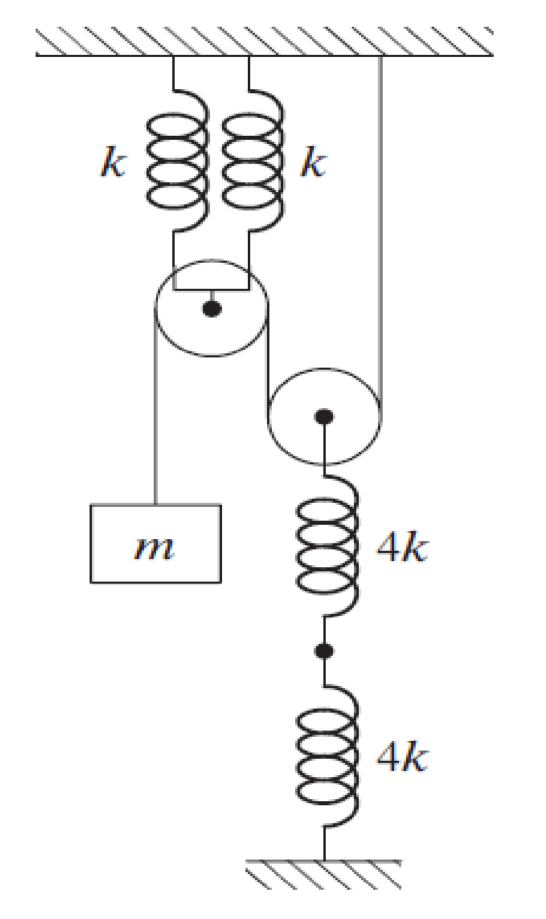
\includegraphics[height=0.60\textwidth]{./problem1b}
\caption[Drawing of  Problem 1(b)]{Drawing of Problem 1(b)}
\label{fig:problem1b}
\end{figure}
\begin{figure}[ht!]
\centering
\def\svgwidth{0.8\textwidth}
\input{problem1b-1.eps_tex}
\caption{Problem geometry}
\end{figure}
~\\
For the fixed length rope:
\begin{eqnarray*}
s_r=\left(L-h_1\right)+h_2-h_1+h_2-h_m=const
\end{eqnarray*}
the relation between the displacements of pulleys is found as using the fixed length rope
\begin{eqnarray*}
\delta s_r =-\delta h_1+\delta h_2-\delta h_1 -\delta h_m=0
\end{eqnarray*}
the relation is found as
\begin{eqnarray*}
\delta h_m =2\delta h_2 -2 \delta h_1\Rightarrow u_m=2\left( u_2- u_1\right)
\end{eqnarray*}
Another relation can be found from the force equilibriums of the pulleys.
From equilibrium of the first pulley with considering serial connected springs, as in fig.\ref{fig:problem1b-2},
\begin{figure}[ht!]
\centering
\def\svgwidth{0.5\textwidth}
\input{problem1b-2.eps_tex}
\caption{Force equilibrium of the first pulley}
\label{fig:problem1b-2}
\end{figure}
\begin{figure}[ht!]
\centering
\def\svgwidth{0.5\textwidth}
\input{problem1b-3.eps_tex}
\caption{Force equilibrium of the second pulley}
\label{fig:problem1b-3}
\end{figure}
\begin{eqnarray*}
2T+2ku_1=0\\
T=-ku_1
\end{eqnarray*}
and from the equilibrium of the second pulley, as in fig.\ref{fig:problem1b-3},
\begin{eqnarray*}
2T-2ku_2=0\\
T=k u_2
\end{eqnarray*}
The relationship
\begin{eqnarray*}
k u_2 =-k u_1 \\
u_2=-u_1
\end{eqnarray*}
using the first and the last displacement relations the system can be reduced to one degree of freedom as
\begin{eqnarray*}
u_2=-\frac{1}{4}u_m
\end{eqnarray*}
Tension on the rod found in terms of $u_m$ as
\begin{eqnarray*}
T=\frac{k}{4} u_m
\end{eqnarray*}
\textbf{The equations of motion using Newton's approach:}\\
\begin{eqnarray*}
-T+mg=m\ddot{u}_m
\end{eqnarray*}
\begin{eqnarray*}
\ddot{u}_m+\frac{k}{4m}u_m=g
\end{eqnarray*}
\textbf{Equations of motion using Lagrange's approach:}
\begin{eqnarray*}
\mathcal{L}=T-V
\end{eqnarray*}
\begin{eqnarray*}
T=\frac{1}{2} m \dot{u}_m^2
\end{eqnarray*}
\begin{eqnarray*}
V=\frac{1}{2}\left(2k\right)u_1^2+\frac{1}{2}\left(2k\right)u_2^2-mgu_m=\frac{1}{2}\left(2k\right)\frac{u_m^2}{16}+\frac{1}{2}\left(2k\right)\frac{u_m^2}{16}-mgu_m
\end{eqnarray*}
\begin{eqnarray*}
\mathcal{L}=T-V=\frac{1}{2}m \dot{u}_m^2-\frac{k}{8}u_m^2+mgu_m
\end{eqnarray*}
\begin{eqnarray*}
\quad \frac{d \left(\frac{\partial \mathcal{L}}{\partial \dot{u}_m}\right)}{dt} -\frac{\partial \mathcal{L}}{\partial {u}_m}=0
\end{eqnarray*}
\begin{eqnarray*}
\ddot{u}_m+\frac{k}{4m}u_m=g
\end{eqnarray*}

\subsection*{c)}
\begin{figure}[ht!]
\centering
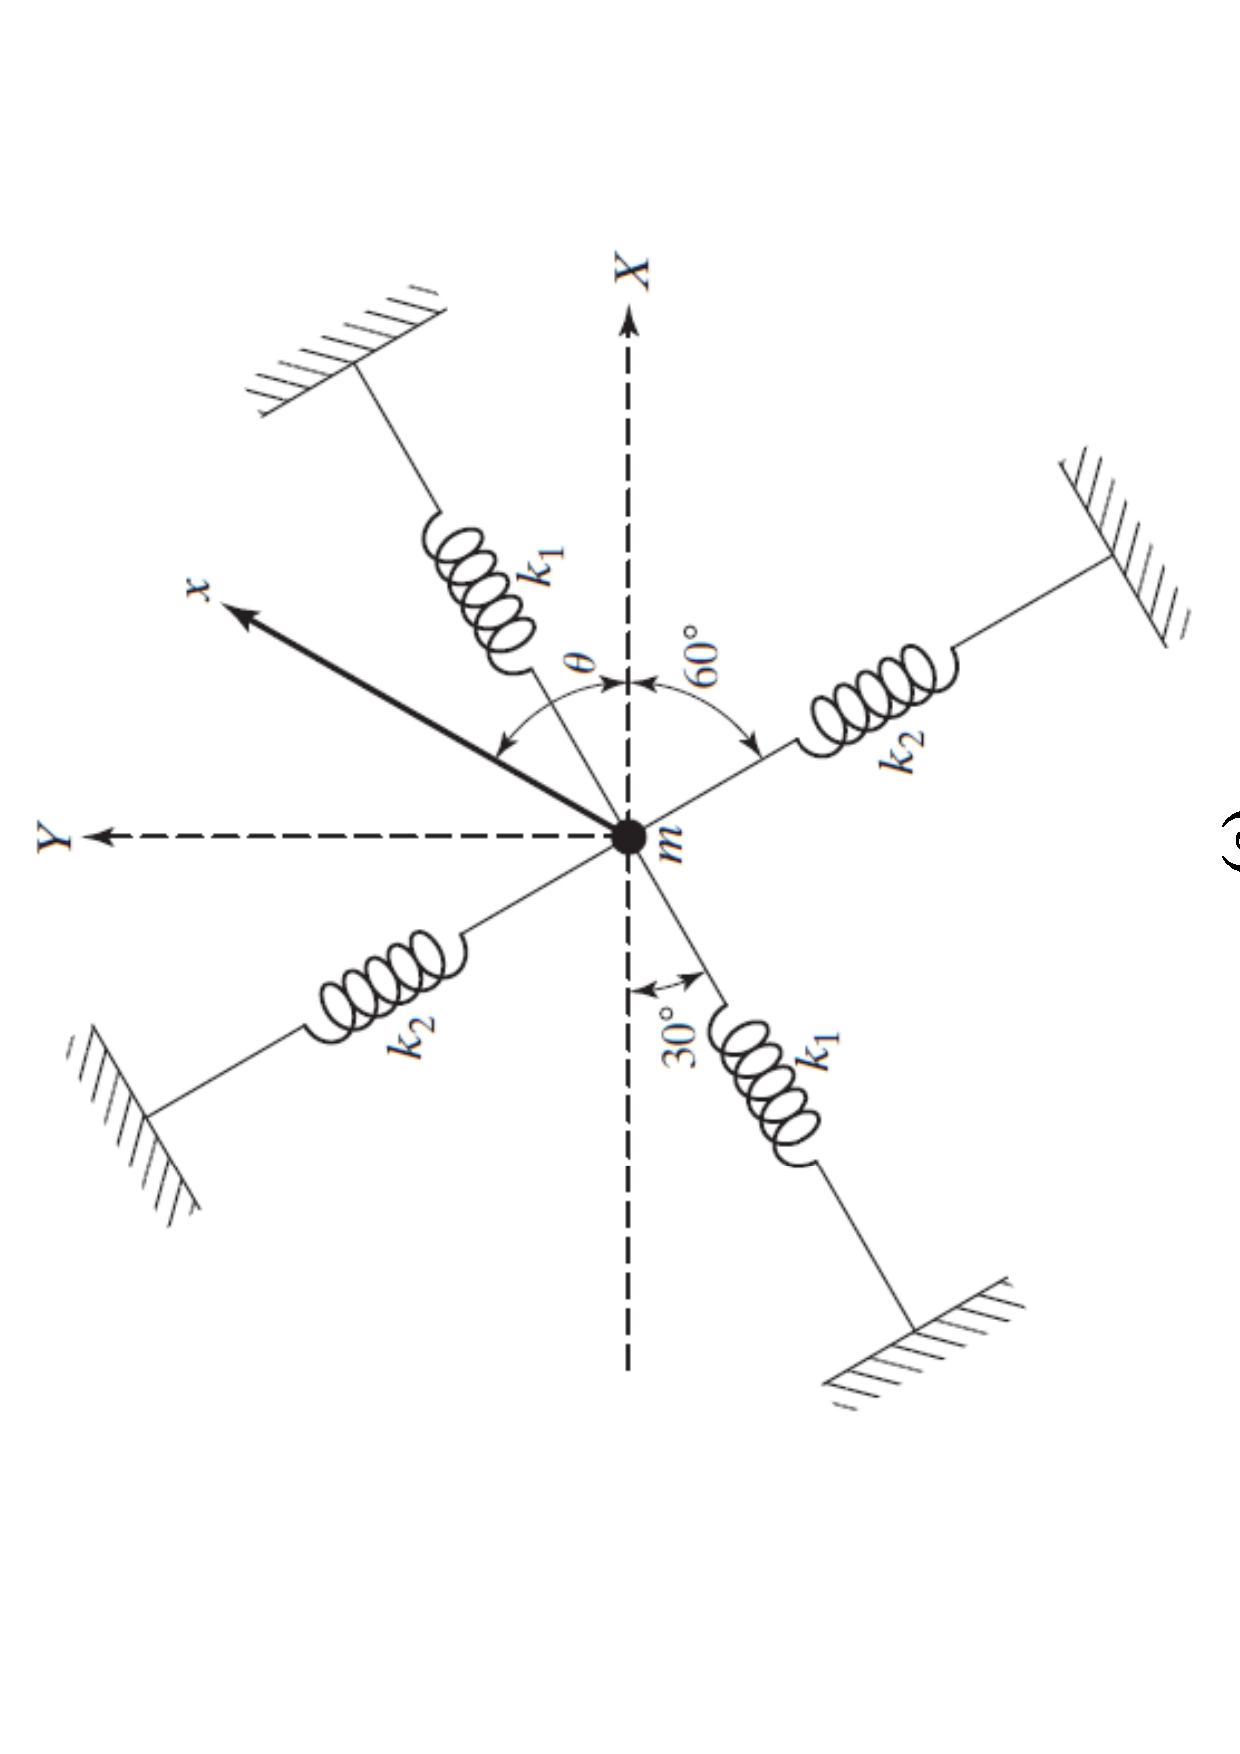
\includegraphics[width=0.5\linewidth,angle=-90]{./problem1c}
\caption{}
\label{fig:problem1c}
\end{figure}
~\\
For the derivation of equation of motion we should apply arbitrary displacement for the mass $m$;
\begin{eqnarray*}
\mathbf{u}_m= u_x \mathbf{i}+u_y \mathbf{j}
\end{eqnarray*}
initial vectorial difference of the springs two ends;
\begin{eqnarray*}
\mathbf{r}_1= -r_x \mathbf{i}-r_y \mathbf{j}
\end{eqnarray*}
\begin{eqnarray*}
\mathbf{r}_2= -r_x \mathbf{i}+r_y \mathbf{j}
\end{eqnarray*}
\begin{eqnarray*}
\mathbf{r}_3= r^{'}_x \mathbf{i}+{r^{'}_y} \mathbf{j}
\end{eqnarray*}
\begin{eqnarray*}
\mathbf{r}_4= -r^{'}_x \mathbf{i}+{r^{'}_y} \mathbf{j}
\end{eqnarray*}
here ;
\begin{eqnarray*}
{r}_x= l_0 \cos{30} &,&r_y= l_0 \sin{30}\\
r^{'}_x= l_0 \cos{60} &,&r^{'}_y= l_0 \sin{60}
\end{eqnarray*}
after deformation,
\begin{eqnarray*}
\left(\mathbf{r}_1\right)_{ad}&=&{\left(-r_x+u_x\right)} \mathbf{i}+{\left(-r_y+u_y\right)} \mathbf{j}\\
\left(\mathbf{r}_2\right)_{ad}&=&{\left(r_x+u_x\right)} \mathbf{i}+{\left(r_y+u_y\right)} \mathbf{j}\\
\left(\mathbf{r}_3\right)_{ad}&=&{\left(-r^{'}_x+u_x\right)} \mathbf{i}+{\left(-r^{'}_y+u_y\right)} \mathbf{j}\\
\left(\mathbf{r}_4\right)_{ad}&=&{\left(r^{'}_x+u_x\right)} \mathbf{i}+{\left(r^{'}_y+u_y\right)} \mathbf{j}
\end{eqnarray*}
\underline{Change on the length of the springs can be found as:}
\begin{eqnarray*}
\Delta l_1 &=&\sqrt{\left(\mathbf{r}_1\right)_{ad}\cdot\left(\mathbf{r}_1\right)_{ad}} -l_0\\
&=&\sqrt{\left(-r_x+u_x\right)^2+\left(-r_y+u_y\right)^2}-l_0\\
&=&\sqrt{-r_x^2-2r_x u_x+u_x^2+r_y^2-2r_y u_y+u_y^2}-l_0\\
&=&\sqrt{l_0^2-2l_0 \cos{30} u_x+u_x^2-2 l_0 \sin{30} u_y+u_y^2}-l_0
\end{eqnarray*}
\begin{eqnarray*}
\Delta l_2 &=&\sqrt{\left(\mathbf{r}_2\right)_{ad}\cdot\left(\mathbf{r}_2\right)_{ad}} -l_0\\
&=&\sqrt{\left(r_x+u_x\right)^2+\left(r_y+u_y\right)^2}-l_0\\
&=&\sqrt{r_x^2+2r_x u_x+u_x^2+r_y^2+2r_y u_y+u_y^2}-l_0\\
&=&\sqrt{l_0^2+2l_0 \cos{30} u_x+u_x^2+2 l_0 \sin{30} u_y+u_y^2}-l_0
\end{eqnarray*}
\begin{eqnarray*}
\Delta l_3 &=&\sqrt{\left(\mathbf{r}_3\right)_{ad}\cdot\left(\mathbf{r}_3\right)_{ad}} -l_0\\
&=&\sqrt{\left(r^{'}_x+u_x\right)^2+\left(r^{'}_y+u_y\right)^2}-l_0\\
&=&\sqrt{ {r^{'}_x}^2+2r^{'}_x u_x+u_x^2+{r^{'}_y}^2+2 r^{'}_y u_y+u_y^2}-l_0\\
&=&\sqrt{l_0^2+2l_0 \cos{60} u_x+u_x^2+2 l_0 \sin{60} u_y+u_y^2}-l_0
\end{eqnarray*}
\begin{eqnarray*}
\Delta l_4 &=&\sqrt{\left(\mathbf{r}_2\right)_{ad}\cdot\left(\mathbf{r}_2\right)_{ad}} -l_0\\
&=&\sqrt{\left(r^{'}_x+u_x\right)^2+\left(r^{'}_y+u_y\right)^2}-l_0\\
&=&\sqrt{{r^{'}_x}^2+2r_x u_x+u_x^2+{r^{'}_y}^2+2r^{'}_y u_y+u_y^2}-l_0\\
&=&\sqrt{l_0^2+2l_0 \cos{60} u_x+u_x^2+2 l_0 \sin{60} u_y+u_y^2}-l_0
\end{eqnarray*}
If we use Langrange's approach to find the equations of motion
\begin{eqnarray*}
\mathcal{L}=T-V
\end{eqnarray*}
\begin{eqnarray*}
T=\frac{1}{2}m\left(\dot{u}_x^2+\dot{u}_y^2\right)
\end{eqnarray*}
\begin{eqnarray*}
V=\frac{1}{2} k_1 \left({\Delta l_1}\right)^2+\frac{1}{2} k_2 \left({\Delta l_2}\right)^2+\frac{1}{2} k_3 \left({\Delta l_3}\right)^2+\frac{1}{2} k_4 \left({\Delta l_4}\right)^2+mg u_y
\end{eqnarray*}
\begin{eqnarray*}
\lefteqn{V=\frac{1}{2} k_1 \biggl({l_0^2-2l_0 \cos{30} u_x+u_x^2-2 l_0 \sin{30} u_y+u_y^2-}
}\\
&&2l_0 \sqrt{{l_0^2-2l_0 \cos{30} u_x+u_x^2-2 l_0 \sin{30} u_y+u_y^2}-l_0} -l_0^2\biggr)\\
&&+\frac{1}{2} k_2 \biggl({l_0^2+2l_0 \cos{30} u_x+u_x^2+2 l_0 \sin{30} u_y+u_y^2-}\\
&& 2l_0 \sqrt{{l_0^2+2l_0 \cos{30} u_x+u_x^2+2 l_0 \sin{30} u_y+u_y^2}} -l_0^2\biggr)\\
&&+\frac{1}{2} k_3 \biggl({l_0^2+2l_0 \cos{60} u_x+u_x^2+2 l_0 \sin{60} u_y+u_y^2-}\\
&& 2l_0 \sqrt{{l_0^2+2l_0 \cos{60} u_x+u_x^2+2 l_0 \sin{60} u_y+u_y^2}} -l_0^2\biggr)
\end{eqnarray*}
In the absence of external forces; Lagrange's equations of motion are
\begin{eqnarray*}
\quad \frac{d \left(\frac{\partial \mathcal{L}}{\partial \dot{\mathbf{q}}}\right)}{dt} -\frac{\partial \mathcal{L}}{\partial \mathbf{q}}=\mathbf{0}
\end{eqnarray*}
By using coordinates as $q_1=u_x$ and $q_2=u_y$\\
\\
\underline{the derivatives of the kinetic energy:}
\begin{eqnarray*}
\frac{ \partial \mathcal{L}}{\partial{\dot{u}_x}}=m \dot{u}_x&,&\frac{\dif\left({\frac{\partial \mathcal{L}}{\partial{\dot{u}_x}}}\right)}{\dif t}=m \ddot{u}_x
\end{eqnarray*}
\begin{eqnarray*}
\frac{ \partial \mathcal{L}}{\partial{\dot{u}_y}}=m \dot{u}_y&,&\frac{\dif\left({\frac{\partial \mathcal{L}}{\partial{\dot{u}_y}}}\right)}{\dif t}=m \ddot{u}_y
\end{eqnarray*}\\
\underline{the derivatives of the potential energy:}\\
\\
\begin{eqnarray*}
\frac{ \partial V}{\partial{u_x}}= k_1  \Delta{l_1}\frac{\partial{\Delta{l_1}}}{\partial{u}_x}+ k_2  \Delta{l_2}\frac{\partial{\Delta{l_2}}}{\partial{u}_x}+ k_3  \Delta{l_3}\frac{\partial{\Delta{l_4}}}{\partial{u}_x}+k_4  \Delta{l_1}\frac{\partial{\Delta{l_4}}}{\partial{u}_x}+0
\end{eqnarray*}
\begin{eqnarray*}
\frac{ \partial V}{\partial{u_y}}= k_1  \Delta{l_1}\frac{\partial{\Delta{l_1}}}{\partial{u}_y}+ k_2  \Delta{l_2}\frac{\partial{\Delta{l_2}}}{\partial{u}_y}+ k_3  \Delta{l_3}\frac{\partial{\Delta{l_4}}}{\partial{u}_y}+k_4  \Delta{l_1}\frac{\partial{\Delta{l_4}}}{\partial{u}_y}+mg
\end{eqnarray*}\\
\underline{The resulting equations of motion are:}\\
\\
\begin{eqnarray*}
\left(1\right)& m\ddot{u}_x+\frac{1}{2}k_1 \left[-2l_0 \cos{30}+2u_x+ \frac{4 l_0^2 \cos{30}}{\sqrt{{l_0^2-2l_0 \cos{30} u_x+u_x^2-2 l_0 \sin{30} u_y+u_y^2}-l_0}}\right]\\
& +\frac{1}{2}k_2 \left[2l_0 \cos{30}+2u_x- \frac{4 l_0^2 \cos{30}}{\sqrt{{l_0^2+2l_0 \cos{30} u_x+u_x^2+2 l_0 \sin{30} u_y+u_y^2}-l_0}}\right]\\
&+\frac{1}{2}k_3 \left[2l_0 \cos{60}+2u_x- \frac{4 l_0^2 \cos{60}}{\sqrt{{l_0^2+2l_0 \cos{30} u_x+u_x^2-2 l_0 \sin{60} u_y+u_y^2}-l_0}}\right]\\
&+\frac{1}{2}k_4 \left[-2l_0 \cos{60}+2u_x+ \frac{4 l_0^2 \cos{60}}{\sqrt{{l_0^2-2l_0 \cos{60} u_x+u_x^2+2 l_0 \sin{60} u_y+u_y^2}-l_0}}\right]=0
\end{eqnarray*}
\\
\begin{eqnarray*}
\left(2\right)& m\ddot{u}_y+\frac{1}{2}k_1 \left[-2l_0 \sin{30}+2u_y+ \frac{4 l_0^2 \cos{30}}{\sqrt{{l_0^2-2l_0 \cos{30} u_x+u_x^2-2 l_0 \sin{30} u_y+u_y^2}-l_0}}\right]\\
& +\frac{1}{2}k_2 \left[2l_0 \sin{30}+2u_y- \frac{4 l_0^2 \cos{30}}{\sqrt{{l_0^2+2l_0 \cos{30} u_x+u_x^2+2 l_0 \sin{30} u_y+u_y^2}-l_0}}\right]\\
&+\frac{1}{2}k_3 \left[-2l_0 \sin{60}+2u_y+ \frac{4 l_0^2 \cos{60}}{\sqrt{{l_0^2+2l_0 \cos{30} u_x+u_x^2-2 l_0 \sin{60} u_y+u_y^2}-l_0}}\right]\\
&+\frac{1}{2}k_4 \left[2l_0 \sin{60}+2u_y- \frac{4 l_0^2 \cos{60}}{\sqrt{{l_0^2-2l_0 \cos{60} u_x+u_x^2+2 l_0 \sin{60} u_y+u_y^2}-l_0}}\right]=-mg
\end{eqnarray*}

\section*{Solution of problem 2}
\begin{figure}[th]
\centering
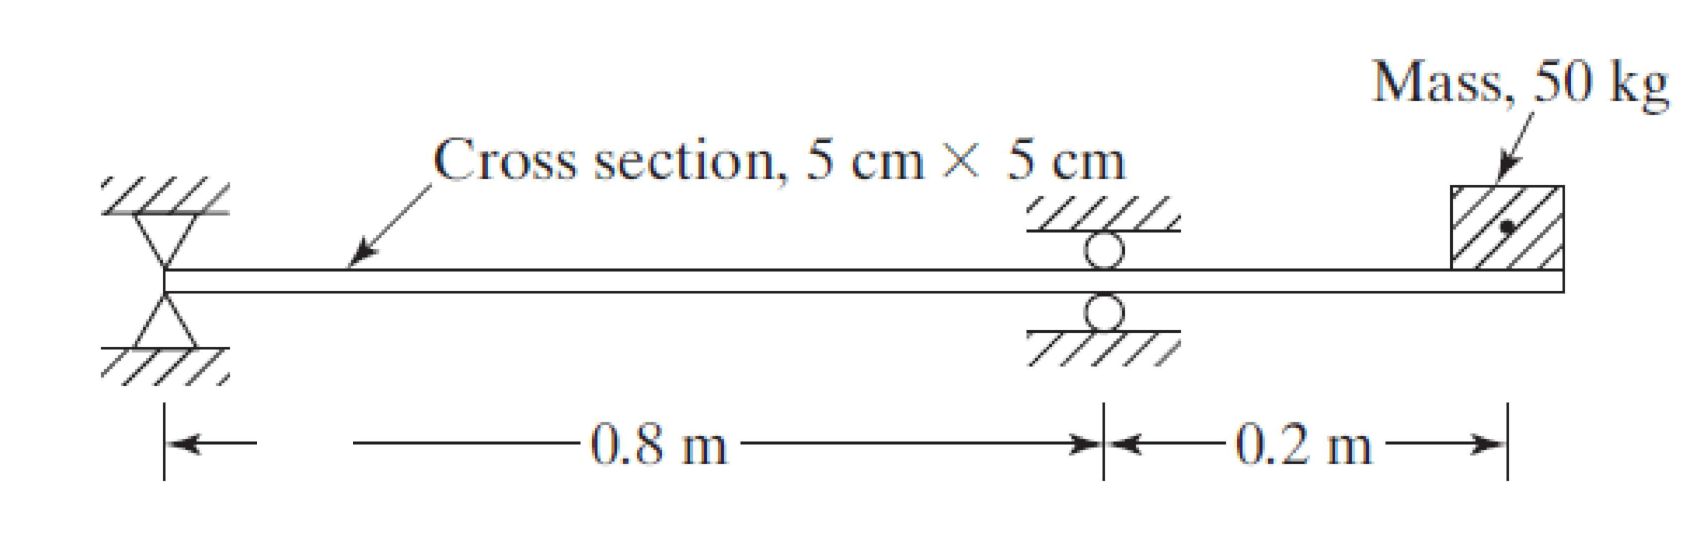
\includegraphics[width=1\linewidth]{./problem2}
\caption[Drawing of problem 2]{Drawing of problem 2}
\label{fig:problem2}
\end{figure}
~\\
Before deriving the equations of motion, whole beam should be treated as a single spring lumped at the tip point. The equavialent model is given in fig.\ref{fig:problem2-equivalentmodel}.
\begin{figure}[th!]
\centering
\begin{pspicture}[xunit=1,yunit=1](0,-3)(5,5)
\psframe(1,1)(4,4)
\pszigzag[coilwidth=0.5,coilheight=1.5,tbarsize=3]{-|}(2.5,1)(2.5,-3)
\rput{0}(2.5,2.5){\psframebox*{m}}
\rput{0}(3.3,-1){\psframebox*{k}}
\end{pspicture}

\caption[Equivalent model of problem 2]{Equivalent model of problem 2}
\label{fig:problem2-equivalentmodel}
\end{figure}
\newline
For the pinned-pinned system that is given in \cite{meirovitch2010fundamentals}, the coefficient of the lumped spring is found as
\begin{eqnarray*}
k=\frac{3EI}{a^2\left(l+a\right)}\quad , \quad I=\frac{1}{12} b h^3=\frac{1}{12} 5. \;5^3=\frac{5^4}{12}
\end{eqnarray*}
\begin{eqnarray*}
k=\frac{3EI}{a^2\left(l+a\right)}=2636718.75\; \text{N/m}
\end{eqnarray*}
Therefore, the equation of motion is found as
\begin{eqnarray*}
m \ddot{u}+ku=0
\end{eqnarray*}
\begin{eqnarray*}
\ddot{u}+\left(229.639\right)^2 u=0
\end{eqnarray*}
where $229.639$ is the natural frequency of the system.
\\
\section*{Solution of problem 3}
\begin{figure}[th!]
\centering
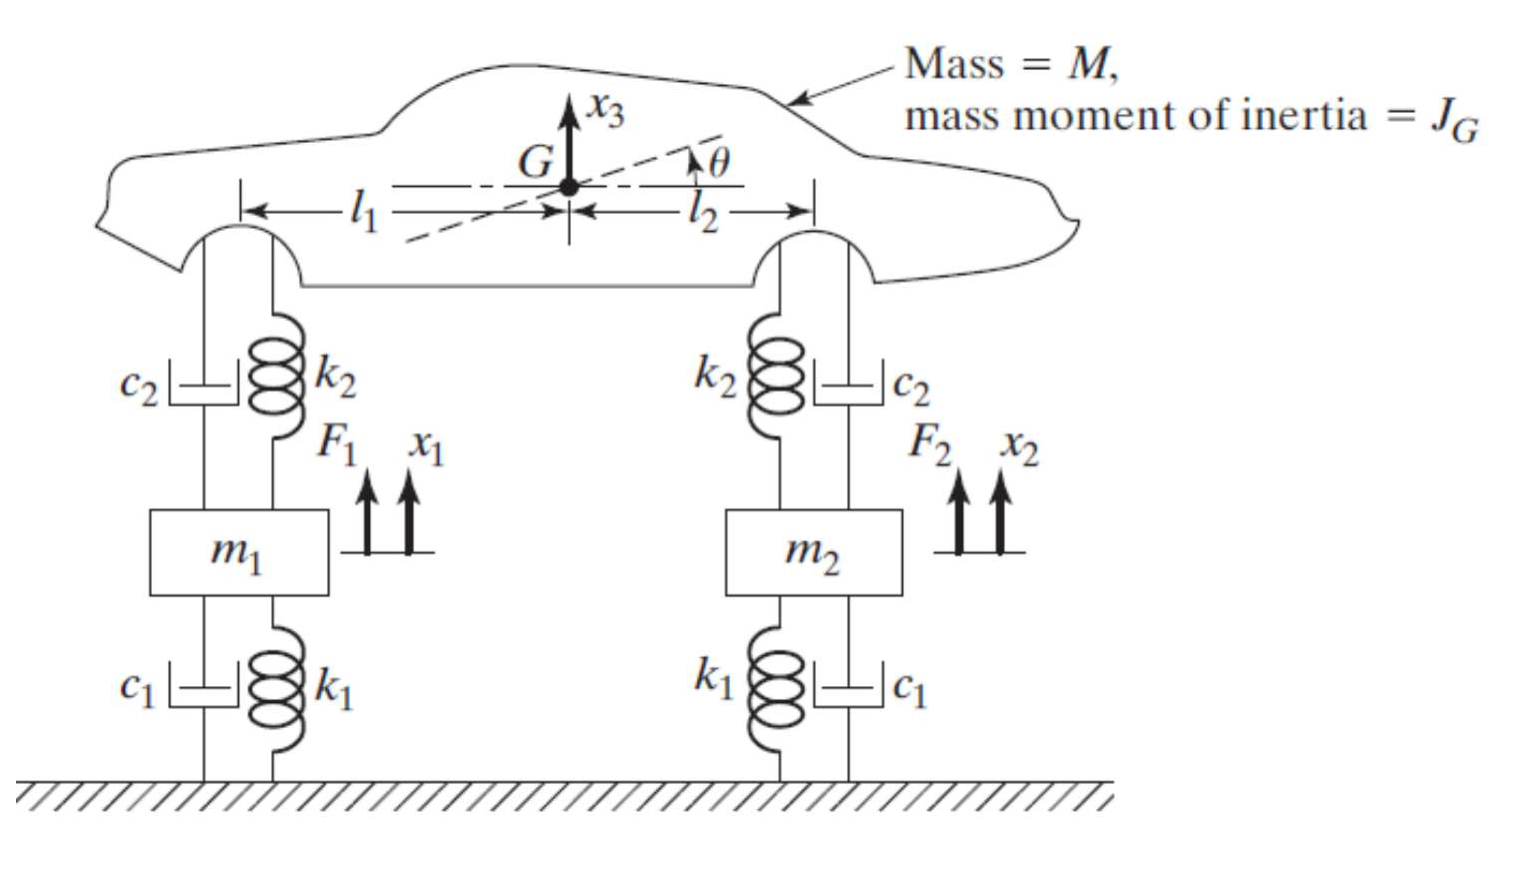
\includegraphics[width=\linewidth]{./problem3}
\caption[Drawing of the problem 3]{Drawing of the problem 3}
\label{fig:problem3}
\end{figure}
~\\
\underline{Derivation of the equations of motion}\\
\\
The system has 4 dof. Therefore, the equations of motion should include four independent equations. The variables are chosen to be rotation of the car $\theta$ and the displacement of the car $u_3$ and displacement of the masses $u_1$ and $u_2$.\\
\\
The displacements of the joint point of the suspension of the car with respect to the orientation  found as

\begin{eqnarray*}
u_{c2}=u_3+l_2 \sin{\theta} \quad ,\quad \dot{u}_{c2}=\dot{u}_3+l_2 \dot{\theta} \cos{\theta} \\
u_{c1}=u_3-l_1 \sin{\theta} \quad ,\quad \dot{u}_{c1}=\dot{u}_3-l_1 \dot{\theta} \cos{\theta}  
\end{eqnarray*}\\
\\
\textbf{Equations of motion using Newton's approach:}\\
\\
Equations of motion of the car is written as
\begin{eqnarray*}
\sum F_3 =M \ddot{u}_3=-k_2\left(\left(u_3-l_1 \sin{\theta}\right) -u_1\right)-c_2\left(\left(\dot{u}_3 -l_1 \dot{\theta} \cos{\theta}\right)-\dot{u}_1\right)-\\
k_2\left(\left(u_3+l_2 \sin{\theta}\right) -u_2\right)-c_2\left(\left(\dot{u}_3 +l_2 \dot{\theta} \cos{\theta}\right)-\dot{u}_2\right)=-Mg
\end{eqnarray*}
\begin{eqnarray*}
\sum M =J_g \ddot{\theta}=l_1 \cos{\theta} \left[ k_2\left(\left(u_3-l_1 \sin{\theta}\right) -u_1\right)+c_2\left(\left(\dot{u}_3 -l_1 \dot{\theta} \cos{\theta}\right)-\dot{u}_1 \right) \right]-\\
l_2 \cos{\theta} \left[k_2\left(\left(u_3+l_2 \sin{\theta}\right) -u_2\right)-c_2\left(\left(\dot{u}_3 +l_2 \dot{\theta} \cos{\theta}\right)-\dot{u}_2\right)\right]
\end{eqnarray*}
and the equations of motion for the masses
\begin{eqnarray*}
\sum F_1 = m_1 \ddot{u}_1=-k_1 u_1 -c_1\dot{u}_1+k_2\left(\left(u_3-l_1\sin{\theta}\right)-u_1\right)-m_1g
\end{eqnarray*}
\begin{eqnarray*}
\sum F_2 = m_2 \ddot{u}_2=-k_1 u_2 -c_1\dot{u}_2+k_2\left(\left(u_3+l_2\sin{\theta}\right)-u_2\right)-m_2g
\end{eqnarray*}
\underline{writing all the equations}
\begin{eqnarray}
M \ddot{u}_3+k_2\left(\left(u_3-l_1 \sin{\theta}\right) -u_1\right)+c_2\left(\left(\dot{u}_3 -l_1 \dot{\theta} \cos{\theta}\right)-\dot{u}_1\right)+\nonumber\\
k_2\left(\left(u_3+l_2 \sin{\theta}\right) -u_2\right)+c_2\left(\left(\dot{u}_3 +l_2 \dot{\theta} \cos{\theta}\right)-\dot{u}_2\right)=-Mg\\
J_g \ddot{\theta}-l_1 \cos{\theta} \left[ k_2\left(\left(u_3-l_1 \sin{\theta}\right) -u_1\right)+c_2\left(\left(\dot{u}_3 -l_1 \dot{\theta} \cos{\theta}\right)-\dot{u}_1 \right) \right]+\nonumber\\
l_2 \cos{\theta} \left[k_2\left(\left(u_3+l_2 \sin{\theta}\right) -u_2\right)-c_2\left(\left(\dot{u}_3 +l_2 \dot{\theta} \cos{\theta}\right)-\dot{u}_2\right)\right]=0\\
 m_1 \ddot{u}_1+k_1 u_1 +c_1\dot{u}_1-k_1\left(\left(u_3-l_1\sin{\theta}\right)-u_1\right)-c_2\left(\left(\dot{u}_3 -l_1 \dot{\theta} \cos{\theta}\right)-\dot{u}_1 \right)=-m_1g\\
m_2 \ddot{u}_2+k_1 u_2 +c_1\dot{u}_2-k_2\left(\left(u_3+l_2\sin{\theta}\right)-u_2\right)-c_2\left(\left(\dot{u}_3 +l_2 \dot{\theta} \cos{\theta}\right)-\dot{u}_2 \right)=-m_2g
\end{eqnarray}
\textbf{Equations of motion using Lagrange's appraoch:}\\
\\
Kinetic energy of the system
\begin{eqnarray*}
T=\frac{1}{2}M\dot{u}_3^2+\frac{1}{2}J_g \dot{\theta}^2+\frac{1}{2}m_1 \dot{u}_1 ^2+\frac{1}{2}m_2 \dot{u}_2^2
\end{eqnarray*}
Potential energy of the system
\begin{eqnarray*}
V&=&\frac{1}{2}k_2 \left(\left(u_3-l_1\sin{\theta}\right)-u_1\right)^2+\frac{1}{2}k_2 \left(\left(u_3+l_2\sin{\theta}\right)-u_2\right)^2+\frac{1}{2}k_1 u_1^2\\ &&+\frac{1}{2}k_2u_2^2+Mgu_3+m_1gu_1+m_2gu_2
\end{eqnarray*}
Virtual work of the damping forces
\begin{eqnarray*}
\delta W =-c_2 \left(\left(\dot{u}_3-l_1 \dot{\theta}\cos{\theta}\right)-\dot{u}_1\right)\delta{\left(\left({u}_3-l_1 \cos{\theta}\right)-{u}_1\right)}-\\
c_2 \left(\left(\dot{u}_3+l_2 \dot{\theta}\cos{\theta}\right)-\dot{u}_2\right)\delta{\left(\left({u}_3+l_2 \cos{\theta}\right)-{u}_2\right)}
-c_1 \dot{u}_1\delta u_1 -c_1 \dot{u}_2 \delta u_2
\end{eqnarray*}
\begin{eqnarray*}
&=&\left[-c_2 \left(\left(\dot{u}_3-l_1 \dot{\theta}\cos{\theta}\right)-\dot{u}_1\right)-
c_2 \left(\left(\dot{u}_3+l_2 \dot{\theta}\cos{\theta}\right)-\dot{u}_2\right)\right]\delta u_3\\
&&+\left[c_2 \left(\left(\dot{u}_3-l_1 \dot{\theta}\cos{\theta}\right)-\dot{u}_1\right)-c_1 \dot{u}_1\right]\delta u_1\\
&&+\left[c_2 \left(\left(\dot{u}_3+l_2 \dot{\theta}\cos{\theta}\right)-\dot{u}_2\right)-c_1 \dot{u}_2\right]\delta u_2\\
&&+\left[c_2 \left(\left(\dot{u}_3-l_1 \dot{\theta}\cos{\theta}\right)-\dot{u}_1\right)l_1 \cos{\theta}-
c_2 \left(\left(\dot{u}_3+l_2 \dot{\theta}\cos{\theta}\right)-\dot{u}_2\right)l_2 \cos{\theta}\right]\delta \theta
\end{eqnarray*}
Lagrange's equations of motion are
\begin{eqnarray*}
\quad \frac{d \left(\frac{\partial \mathcal{L}}{\partial \dot{\mathbf{q}}}\right)}{dt} -\frac{\partial \mathcal{L}}{\partial \mathbf{q}}=\mathbf{Q}_e
\end{eqnarray*}
Required derivatives for the equations of motion using Lagrange's approach:\\
\\
First, derivatives related to coordinate velocities,
\begin{eqnarray*}
\frac{\partial \mathcal{L}}{\partial \dot{u}_1}=m_1 \dot{u}_1 \;,\; \frac{\partial \mathcal{L}}{\dot{u}_2}=m_2 \dot{u}_2 \;,\; \frac{\partial \mathcal{L}}{\partial \dot{u}_3}=M\dot{u}_3 \;,\;\frac{\partial \mathcal{L}}{\partial \dot{\theta}}=J_g \dot{\theta}
\end{eqnarray*}
and their exact differentials ratio with respect to time $t$
\begin{eqnarray*}
\frac{d\left(\frac{\partial \mathcal{L}}{\partial \dot{u}_1}\right)}{d t}=m_1 \ddot{u}_1 \;,\; \frac{d\left(\frac{\partial \mathcal{L}}{\partial \dot{u}_2}\right)}{d t}=m_2 \ddot{u}_2 \;,\; \frac{d\left(\frac{\partial \mathcal{L}}{\partial \dot{u}_3}\right)}{d t}=M\ddot{u}_3 \;,\;\frac{d\left(\frac{\partial \mathcal{L}}{\partial \dot{\theta}}\right)}{d t}=J_g \ddot{\theta}
\end{eqnarray*}
then derivatives related to coordinates itself,
\begin{eqnarray*}
\frac{\partial \mathcal{L}}{\partial {u}_1}=k_2\left(\left(u_3 -l_1 \sin{\theta}\right)-u_1\right)-k_1u_1-m_1 g \\
\frac{\partial \mathcal{L}}{\partial {u}_2}=k_2\left(\left(u_3 +l_2 \sin{\theta}\right)-u_2\right)-k_2u_2-m_2 g\\
\frac{\partial \mathcal{L}}{\partial {u}_3}=-k_2 \left(\left(u_3 -l_1 \sin{\theta}\right)-u_1\right)-k_2\left(\left(u_3 +l_2 \sin{\theta}\right)-u_2\right)-M g \\
\frac{\partial \mathcal{L}}{\partial \theta}=k_2\left(\left(u_3 -l_1 \sin{\theta}\right)-u_1\right) \cos{\theta}-k_2\left(\left(u_3 +l_2 \sin{\theta}\right)-u_2\right) \cos{\theta}
\end{eqnarray*}
The equations of motion are found by plugging derivatives into Lagrange's equations of motion for all independent coordinates :\\
\\
\underline{For $u_1$:}
\begin{eqnarray*}
m_1 \ddot{u}_1-k_2\left(\left(u_3 -l_1 \sin{\theta}\right)-u_1\right)+k_1u_1+m_1 g=c_2 \left(\left(\dot{u}_3-l_1 \dot{\theta}\cos{\theta}\right)-\dot{u}_2\right)-c_1 \dot{u}_1
\end{eqnarray*}\\
\\
\underline{For $u_2$:}
\begin{eqnarray*}
m_2 \ddot{u}_2-k_2\left(\left(u_3+l_2 \sin{\theta}\right)-u_2\right)+k_2u_2+m_2 g=c_2 \left(\left(\dot{u}_3+l_2 \dot{\theta}\cos{\theta}\right)-\dot{u}_2\right)-c_1 \dot{u}_2
\end{eqnarray*}\\
\\
\underline{For $u_3$:}
\begin{eqnarray*}
M \ddot{u}_3+k_2\left(\left(u_3-l_2 \sin{\theta}\right)-u_1\right)+k_2\left(\left(u_3+l_2 \sin{\theta}\right)-u_2\right)- M g =\\ -c_2 \left(\left(\dot{u}_3-l_1 \dot{\theta}\cos{\theta}\right)-\dot{u}_1\right)-c_2 \left(\left(\dot{u}_3+l_2 \dot{\theta}\cos{\theta}\right)-\dot{u}_2\right)
\end{eqnarray*}
\underline{For $\theta$:}
\begin{eqnarray*}
J_g \ddot{\theta}-k_2\left(\left(u_3 -l_1 \sin{\theta}\right)-u_1\right) \cos{\theta}+k_2\left(\left(u_3 +l_2 \sin{\theta}\right)-u_2\right) \cos{\theta}=\\
c_2 \left(\left(\dot{u}_3-l_1 \dot{\theta}\cos{\theta}\right)-\dot{u}_1\right)l_1 \cos{\theta}-
c_2 \left(\left(\dot{u}_3+l_2 \dot{\theta}\cos{\theta}\right)-\dot{u}_2\right)l_2 \cos{\theta}
\end{eqnarray*}
\section*{Solution of problem 4}

Solution of this problem requires to use Hamilton's principle since there are infinite generalized coordinates that are required to represent the motion of the beam. The Hamilton's statement in the absence of external forces is
\begin{eqnarray*}
\delta I =\delta \int_{t_1}^{t_2} \left(T-V \right)dt=0
\end{eqnarray*}
Kinetic and potential energy of the system respectively
\begin{eqnarray*}
T= \int_{0}^{L}\frac{1}{2}\rho A \left(x\right) {\left(\frac{\partial{ u\left(x,t\right)}}{\partial{t}}\right)}^2  dx
\end{eqnarray*}
\begin{eqnarray*}
V= \int_{0}^{L}\frac{1}{2} E I {\left(\frac{\partial^2{u\left(x,t\right)}}{\partial{x^2}}\right)}^2 dx+\frac{1}{2}k_t {\theta{\left(0,t\right)}}^2+\frac{1}{2} k {u \left(L,t\right)}^2
\end{eqnarray*}
Substituting both into Hamilton's principle
\begin{eqnarray}
\label{variation_of_functional}
\delta I& =&\delta \int_{t_1}^{t_2}\biggl[\int_{0}^{L}\left(\frac{1}{2}\rho A \left(x\right) {\left(\frac{\partial{ u\left(x,t\right)}}{\partial{t}}\right)}^2 -\frac{1}{2} E I {\left(\frac{\partial^2{u\left(x,t\right)}}{\partial{x^2}}\right)^2}\right) dx \nonumber\\
&&-\frac{1}{2}k_t {\theta{\left(0,t\right)}}^2-\frac{1}{2} k {u \left(L,t\right)}^2\biggr]dt=0
\end{eqnarray}
If we divide variation of the integral into parts as
\begin{eqnarray*}
 \frac{1}{2}\rho A \int_{t1}^{t2} \; \int_{0}^{L} \delta\left( {\left(\frac{\partial{ u\left(x,t\right)}}{\partial{t}}\right)}^2 \right) dx \; dt\qquad\left[1\right] \\
 \frac{1}{2}E I \int_{t1}^{t2} \;\int_{0}^{L}  \delta\left( {\left(\frac{\partial^2{u\left(x,t\right)}}{\partial{x^2}}\right)}^2\right) dx\; dt\qquad\left[2\right]\\
\frac{1}{2}k_t \int_{t1}^{t2} \;\delta \left({\theta{\left(0,t\right)}}^2\right)dt\qquad\left[3\right]\\
\frac{1}{2} k \int_{t1}^{t2} \; \delta \left( {u \left(L,t\right)}^2\right)dt\qquad\left[4\right]
\end{eqnarray*}
\\
\underline{Finding the result of the first term}:\\
\\
by changing the integrand ordering and applying variaton
\begin{eqnarray*}
\frac{1}{2} \rho A \int_{0}^{L}\;  \int_{t1}^{t2}  \delta\left( {\left(\frac{\partial{ u\left(x,t\right)}}{\partial{t}}\right)}^2 \right) dt\;  dx =\rho A \int_{0}^{L}\;  \int_{t1}^{t2} \frac{\partial{ u\left(x,t\right)}}{\partial{t}} \delta {\left(\frac{\partial{ u\left(x,t\right)}}{\partial{t}}\right)}  dt\;  dx
\end{eqnarray*}
since $\delta \left(\frac{\partial{u \left(x,t\right)}}{\partial{t}}\right)=\frac{\partial{\delta u\left(x,t\right)}}{\partial t}$ the first integral can be written as
\begin{eqnarray*}
\int_{t1}^{t2} \frac{\partial{ u\left(x,t\right)}}{\partial{t}}\frac{\partial{\delta u\left(x,t\right)}}{\partial t}  dt=\frac{\partial{ u\left(x,t\right)}}{\partial{t}} \delta u\left(x,t\right) {|}_{t_1}^{t_2}-\int_{t1}^{t2} \frac{\partial^2{ u\left(x,t\right)}}{\partial{t^2}}\delta u\left(x,t\right)dt
\end{eqnarray*}
where $\frac{\partial{ u\left(x,t\right)}}{\partial{t}}=v$ and $\frac{\partial{ \delta u\left(x,t\right)}}{\partial{t}}dt=du$ is used. Therefore,
\begin{equation*}
\begin{split}
\frac{1}{2}\rho A \int_{t1}^{t2} \; \int_{0}^{L} \delta\left( {\left(\frac{\partial{ u\left(x,t\right)}}{\partial{t}}\right)}^2 \right) dx \; dt&= \rho A \int_{0}^{L}\biggl[\frac{\partial{ u\left(x,t\right)}}{\partial{t}} \delta u\left(x,t\right) {|}_{t_1}^{t_2}-\\
&\int_{t1}^{t2} \frac{\partial^2{ u\left(x,t\right)}}{\partial{t^2}}\delta u\left(x,t\right)dt\biggr]dx
 \end{split}
\end{equation*}
By the fixed variation of displacements on the start and end points in time we have $\frac{\partial{ u\left(x,t\right)}}{\partial{t}} \delta u\left(x,t\right) {|}_{t_1}^{t_2}=0$. \\
\\
The result is found as
\begin{eqnarray*}
\frac{1}{2}\rho A \int_{t1}^{t2} \; \int_{0}^{L} \delta\left( {\left(\frac{\partial{ u\left(x,t\right)}}{\partial{t}}\right)}^2 \right) dx \; dt=-\rho A \int_{0}^{L}\int_{t1}^{t2} \frac{\partial^2{ u\left(x,t\right)}}{\partial{t^2}}\delta u\left(x,t\right)dt dx
\end{eqnarray*}
\\
\underline{Finding the result of the second term}:\
\\
\begin{eqnarray*}
\frac{1}{2}E I \int_{t1}^{t2} \;\int_{0}^{L}  \delta\left( {\left(\frac{\partial^2{u\left(x,t\right)}}{\partial{x^2}}\right)}^2\right) dx\; dt= E I \int_{t1}^{t2} \;\int_{0}^{L}   \frac{\partial^2{u\left(x,t\right)}}{\partial{x^2}} \delta{\left(\frac{\partial^2{u\left(x,t\right)}}{\partial{x^2}}\right)} dx\; dt
\end{eqnarray*}
using  $\delta \left(\frac{\partial^2{u \left(x,t\right)}}{\partial{x^2}}\right)=\frac{\partial^2{\delta u\left(x,t\right)}}{\partial x^2}$ the first integral found as
\begin{eqnarray*}
\int_{0}^{L}   \frac{\partial^2{u\left(x,t\right)}}{\partial{x^2}} \frac{\partial^2{\delta u\left(x,t\right)}}{\partial x^2} dx=    \frac{\partial^2{u\left(x,t\right)}}{\partial{x^2}} \frac{\partial{\delta u\left(x,t\right)}}{\partial x}{|}_{0}^{L}-\int_{0}^{L}   \frac{\partial^3{u\left(x,t\right)}}{\partial{x^3}} \frac{\partial{\delta u\left(x,t\right)}}{\partial x} dx
\end{eqnarray*}
where $\frac{\partial^2{ u\left(x,t\right)}}{\partial{x^2}}=v$ and $\frac{\partial^2{ \delta u\left(x,t\right)}}{\partial{x^2}}dt=du$ is used. Using same approach for the calculation of the term $\int_{0}^{L} \frac{\partial^3{u\left(x,t\right)}}{\partial{x^3}} \frac{\partial{\delta u\left(x,t\right)}}{\partial x} dx$ again 
\begin{eqnarray*}
\int_{0}^{L}   \frac{\partial^3{u\left(x,t\right)}}{\partial{x^3}} \frac{\partial{\delta u\left(x,t\right)}}{\partial x} dx =\frac{\partial^3{u\left(x,t\right)}}{\partial{x^3}} {\delta u\left(x,t\right)}{|}_{0}^{L}-\int_{0}^{L}   \frac{\partial^4{u\left(x,t\right)}}{\partial{x^4}} {\delta u\left(x,t\right)} dx
\end{eqnarray*}
the second term of the eq.\ref{variation_of_functional} is found as
\begin{eqnarray*}
 \lefteqn{\frac{1}{2}E I \int_{t1}^{t2} \;\int_{0}^{L}  \delta\left( {\left(\frac{\partial^2{u\left(x,t\right)}}{\partial{x^2}}\right)}^2\right) dx\; dt=}\\
 & &E I\int_{t1}^{t2} \;\left[ \frac{\partial^2{u\left(x,t\right)}}{\partial{x^2}} \frac{\partial{\delta u\left(x,t\right)}}{\partial x}{|}_{0}^{L}  -\frac{\partial^3{u\left(x,t\right)}}{\partial{x^3}} {\delta u\left(x,t\right)}{|}_{0}^{L} +\int_{0}^{L}   \frac{\partial^4{u\left(x,t\right)}}{\partial{x^4}} {\delta u\left(x,t\right)}dx \right] dt
\end{eqnarray*}
\\
\newpage
~\\
\underline{Finding the result of the third term}:\\
\\
\begin{eqnarray*}
\frac{1}{2}k_t \int_{t1}^{t2} \;\delta \left({\theta{\left(0,t\right)}}^2\right)dt=k_t \int_{t1}^{t2} \;\theta{\left(0,t\right)}\delta {\theta{\left(0,t\right)}}dt
\end{eqnarray*}
for the $\theta{\left(0,t\right)}$:
\begin{eqnarray*}
\tan{\theta{\left(0,t\right)}}=\frac{\partial{u{\left(0,t\right)}}}{\partial{x}}
\end{eqnarray*}
for $\theta{\left(0,t\right)}\approx 0$ it is found that
\begin{eqnarray*}
{\theta{\left(0,t\right)}}=\frac{\partial{u{\left(0,t\right)}}}{\partial{x}}
\end{eqnarray*}
and
\begin{eqnarray*}
\delta \theta{\left(0,t\right)}=\frac{\partial{\delta u{\left(0,t\right)}}}{\partial{x}}
\end{eqnarray*}
The third term, thus, 
\begin{eqnarray*}
\frac{1}{2}k_t \int_{t1}^{t2} \;\delta \left({\theta{\left(0,t\right)}}^2\right)dt=k_t \int_{t1}^{t2} \; \frac{\partial{u{\left(0,t\right)}}}{\partial{x}} \frac{\partial{\delta u{\left(0,t\right)}}}{\partial{x}}dt
\end{eqnarray*}\\
\\
\underline{Finding the result of the fourth term:}\\
\\
\begin{eqnarray*}
\frac{1}{2} k \int_{t1}^{t2} \; \delta \left( {u \left(L,t\right)}^2\right)dt= k \int_{t1}^{t2} \;u \left(L,t\right) \delta  u \left(L,t\right)dt
\end{eqnarray*}
\\
\underline{Last form of eqn.\ref{variation_of_functional}:}\\
\\
Plugging all four terms in eq.\ref{variation_of_functional}, eq.\ref{variation_of_functional} has the form
\begin{eqnarray}
\begin{split}
\delta I &=
\int_{t1}^{t2} \biggl[ \int_{0}^{L}  \left(-\rho A \frac{\partial^2{ u\left(x,t\right)}}{\partial{t^2}} -E I\frac{\partial^4{u\left(x,t\right)}}{\partial{x^4}}\right)  dx\,{\delta u\left(x,t\right)} \\
&+E I\frac{\partial^2{u\left(x,t\right)}}{\partial{x^2}} \frac{\partial{\delta u\left(x,t\right)}}{\partial x}{|}_{0}^{L}\\ 
&-E I\frac{\partial^3{u\left(x,t\right)}}{\partial{x^3}} {\delta u\left(x,t\right)}{|}_{0}^{L} +k_t  \; \frac{\partial{u{\left(0,t\right)}}}{\partial{x}} \frac{\partial{\delta u{\left(0,t\right)}}}{\partial{x}}+k  \;u \left(L,t\right) \delta  u \left(L,t\right) \biggr]dt=0
\end{split}
\end{eqnarray}
Knowing that the any integral $\int_{a}^{b} f\left(\xi\right)d \xi=0$ requires $f\left(\xi\right)$ to be zero we should have
\begin{eqnarray}
\nonumber
&& \int_{0}^{L}  \left(-\rho A \frac{\partial^2{ u\left(x,t\right)}}{\partial{t^2}} -E I\frac{\partial^4{u\left(x,t\right)}}{\partial{x^4}}\right)  dx\,{\delta u\left(x,t\right)} +E I\frac{\partial^2{u\left(x,t\right)}}{\partial{x^2}} \frac{\partial{\delta u\left(x,t\right)}}{\partial x}{|}_{0}^{L}-\\ &&E I\frac{\partial^3{u\left(x,t\right)}}{\partial{x^3}} {\delta u\left(x,t\right)}{|}_{0}^{L} +k_t  \; \frac{\partial{u{\left(0,t\right)}}}{\partial{x}} \frac{\partial{\delta u{\left(0,t\right)}}}{\partial{x}}+k  \;u \left(L,t\right) \delta  u \left(L,t\right) =0\nonumber
\end{eqnarray}
putting the values at $L$ and $0$ and with parenthesizing with respect to variations the resulting equation is
\begin{eqnarray}
\nonumber
\lefteqn{\left[ \int_{0}^{L}  \left(-\rho A \frac{\partial^2{ u\left(x,t\right)}}{\partial{t^2}} -E I\frac{\partial^4{u\left(x,t\right)}}{\partial{x^4}}\right)  dx\, \right]{\delta u\left(x,t\right)} }\\
&&+\left[E I\frac{\partial^2{u\left(L,t\right)}}{\partial{x^2}} \right]\frac{\partial{\delta u\left(L,t\right)}}{\partial x}\nonumber\\ 
&&+\left[E I\frac{\partial^3{u\left(L,t\right)}}{\partial{x^3}}+k u \left(L,t\right) \right] {\delta u\left(L,t\right)}\label{solution4result} \\
&&-\left[E I\frac{\partial^3{u\left(0,t\right)}}{\partial{x^3}} \right] {\delta u\left(0,t\right)}\nonumber\\
&&+\left[E I\frac{\partial^2{u\left(L,t\right)}}{\partial{x^2}} \right]\frac{\partial{\delta u\left(L,t\right)}}{\partial x}\nonumber\\ 
&&+\left[k_t  \; \frac{\partial{u{\left(0,t\right)}}}{\partial{x}} -E I\frac{\partial^2{u\left(0,t\right)}}{\partial{x^2}}\right]\frac{\partial{\delta u{\left(0,t\right)}}}{\partial{x}}  \; =0\nonumber
\end{eqnarray}
Knowing that the variations are arbitrary and independent, their derivatives are also independent, the coefficients of the variations and coefficients of their derivatives should be equal to zero in eq.(\ref{solution4result}). With using the requirement $f\left(\xi\right)=0$ for $\int_{a}^{b} f\left(\xi\right)d \xi=0$ the solution for this problem is
\begin{eqnarray}
-\rho A \frac{\partial^2{ u\left(x,t\right)}}{\partial{t^2}} -E I\frac{\partial^4{u\left(x,t\right)}}{\partial{x^4}}=0 \nonumber & \text{(equations of motion)}
\end{eqnarray}
\begin{eqnarray}
E I\frac{\partial^3{u\left(0,t\right)}}{\partial{x^3}}=0\nonumber & \text{(force free end at $x=0$)}
\end{eqnarray}
\begin{eqnarray}
E I\frac{\partial^2{u\left(L,t\right)}}{\partial{x^2}}=0\nonumber&\text{(Moment free end at $x=L$)}
\end{eqnarray}
\begin{eqnarray} 
E I\frac{\partial^3{u\left(L,t\right)}}{\partial{x^3}}+k u \left(L,t\right) =0\nonumber&
\text{(Force equilibrium at $x=L$)}
\end{eqnarray}
\begin{eqnarray}
k_t  \; \frac{\partial{u{\left(0,t\right)}}}{\partial{x}} -E I\frac{\partial^2{u\left(0,t\right)}}{\partial{x^2}} =0\nonumber&
\text{(Moment equilibrium at $x=0$)}
\end{eqnarray}
\bibliographystyle{plain}
\bibliography{biblio}

\end{document}          


